\chapter{Methodology and Results}
The Riskmap system allows citizens to easily submit
disaster reports. From 2016 to date, the system has allowed the Urban Risk Lab
at MIT (MIT-URL) to gather 2229 reports before, during, and after flood
emergencies in Jakarta. Similarly the Riskmap platform has also gathered 356
reports in Chennai. \figureautorefname{}~\ref{fig:ch_typical_reports} demonstrates
that these data points include traffic reports, indications
that an area is unsafe, and advice for other citizens in the area.  Images
attached to reports include a wide variety of scenes, from daylight-highways
with cars and motorcycles to night time deserted alleys. The data points include
not only textual and image data but also estimated flood heights.

\begin{figure}[ht]
    \centering
    \captionsetup{justification=centering}
    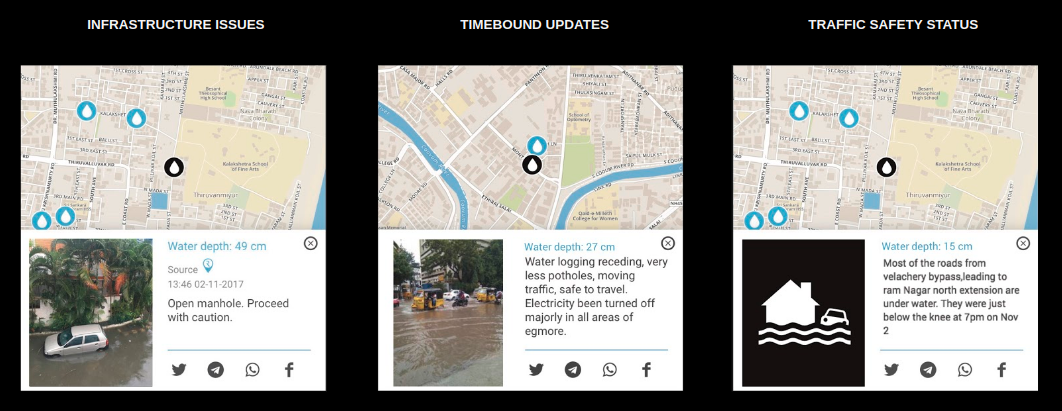
\includegraphics[width=\textwidth]{images/ch/typical_reports.png}
    \caption{Representative reports of heavy flooding in Chennai during Nov.
    2017 Monsoon }\label{fig:ch_typical_reports}
\end{figure}

The disparate datasets contained in the Riskmap System motivate the creation of
REACT in order to process and summarize results in real time.

\section{System Design}
It is paramount for disaster systems to be highly available and scalable during
events. The REACT system has been designed such that it is modular and ready to
scale. A simple but expandable configuration file interface serves as a
singleton for sharing global environment variables such as database connections
and logging capabilities. The DataLoader interface allows for flexibility in the
data source that is used, while the Labeler construct allows one to use
different services to create embeddings of that data. Finally, any class that
follows the Learner specification is able to train and validate on those
embeddings.

\subsection{Configuration}
A single configuration file allows for easy customization of the underlying 
training data. \figureautorefname{}~\ref{fig:config} shows the configuration
abstraction. Two default implementations of this interface include all of the
data from Chennai and Jakarta in 2017. Other configurations allow the
opportunity to choose only those reports that include an image, or those that
come from a specific social network.
\begin{figure}[ht]
    \centering
    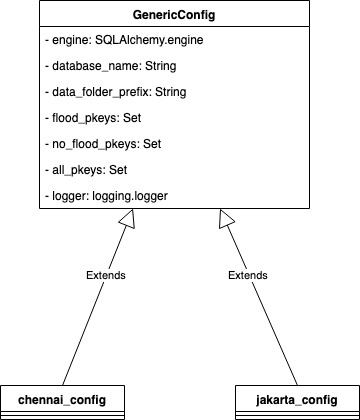
\includegraphics[scale=0.6]{images/config.jpg}
    \caption{Configuration Abstraction}\label{fig:config}
\end{figure}

\subsection{Data Loaders}
Data Loaders are constructed by passing a configuration that implements the 
GenericConfig interface. They are then responsible for implementing methods 
that allow for retrieving the three kinds of data that the REACT system 
uses for prediction: text, image, and flood depth estimation. While the
RiskmapLoader is the only Loader that is currently implemented, it was 
important to separate data loaders in order to make REACT ready for future change.
% TODO talk about japan?
% TODO CITE :https://www.gov-online.go.jp/eng/publicity/book/hlj/html/201803/201803_03_en.html

\begin{figure}[ht]
    \centering
    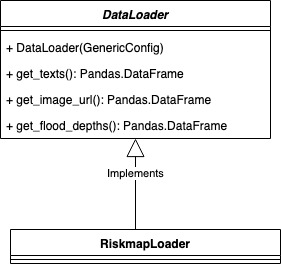
\includegraphics[scale=0.6]{images/loaders.jpg}
    \caption{Adaptable Data Loaders}\label{fig:data_loaders}
\end{figure}

\subsection{Labelers}
Data embeddings, or labels, turn human recognizable data into feature vectors
that can be used for machine learning. There are many choices for how to 
label the disaster data in REACT, as such any Labeler that implements the 
GenericLabeler interface can be used seamlessly in the system as shown in \figureautorefname{}~\ref{fig:labelers}. The AwsLabeler uses AWS Rekognition 
to create feature vectors, while the BowLabeler uses a bag of words approach 
to encode textual information. An IdentityLabeler is provided in order to 
facilitate the passing of raw features.
\begin{figure}[ht]
    \centering
    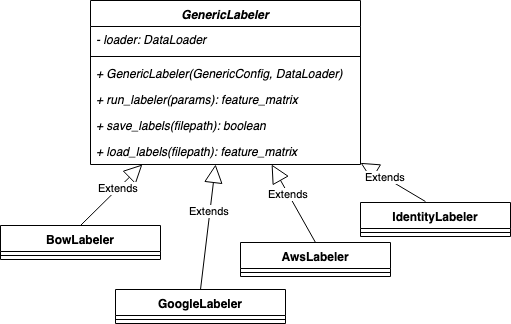
\includegraphics[scale=0.6]{images/labelers.png}
    \caption{Many different labelers can be used to encode data in REACT}\label{fig:labelers}
\end{figure}

\subsection{Learners}
Different learning methods are represented by different implementations of
the GenericLearner interface as shown in
\figureautorefname{}~\ref{fig:labelers}. The perceptron algorithm and the
Support Vector Machine (SVM) method are implemented in REACT as simple linear
classifiers. The perceptron algorithm is an iterative method that tries to find
a separator through simple linear transformations, meanwhile SVMs try to find
the max margin separator by using a squared loss
objective~\cite{bishopPatternRecognitionMachine2006}. An IdentityLearner is also
provided to act as a pass through in case raw features are desired.
\begin{figure}[ht]
    \centering
    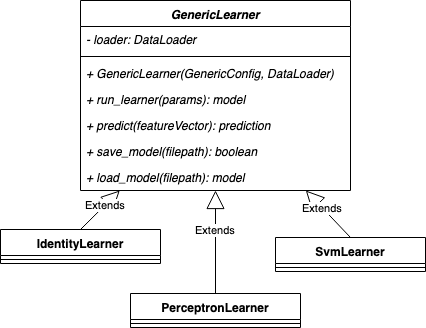
\includegraphics[scale=0.6]{images/learners.png}
    \caption{The Learner abstraction makes it easy to switch from one method to another}\label{fig:learners}
\end{figure}

\section{Ground Truth}~\label{chap4:ground_truth}
We explored two different methods in order to decide whether a particular report
was indicative of heavy flooding or not. We first classified a report as heavy
flooding if it was submitted during a time range when we knew there to be heavy 
flooding in the corresponding city. These shall be referred to as time-classified.
Although we expected this classification to be very coarse, we hoped that it would
be specific enough to create an accurate predictor. In order to test this theory 
we also hand labeled reports by inspecting the images that accompanied them; these
will be referred to as hand-classified. 

\section{Text}
As shown in Section~\ref{chap1:riskmap}, the Riskmap system allows citizens to provide
a textual description to emergency managers. In Indonesia, most of the reports
are provided in Bahasa, the local language; however, in Chennai all reports were
submitted in English even though the system also supports Tamil. In both Chennai
and Jakarta these reports are quite brief, with the longest reports having 140
characters. In this manner, they are quite similar to tweets which were
initially 140 characters but this limit was doubled in 2017. Helpfully, this
means that much of the work described in Section~\ref{chap3:text} applies to the Riskmap
text corpus.

Table~\ref{table:text_sample} contains a sample of ten reports that are
indicative of those found in the Riskmap textual descriptions.

\begin{table}
\centering
  \begin{tabular}{ll}
    \toprule
    pkey & text \\ 
    \hline
    \midrule
    169  &
    Waterlogging near cathedral road flyover  \\
    171  &
    1st street Engineers avenue \\
    173  &
    Not that much water safe only \\
    174  &
    50cm water stagnant on the road \\
    176  &
    Water level rising  slowly  \\
    177  &
    Water logging  \\
    178  &
    Model school road is completely flooded, with water almost knee deep \\
    179  &
    Heavy rain in West mambalam flood \\
    180  &
    Water on roads. Stay safe \\
    182  &                                                           4cm
    rainfall.. still continuing.. hope for safe .. dont come outside in
    night time \\
    181  &
    Luz signal flooded knee deep water \\
    \bottomrule
  \end{tabular}
  \caption{A representative selection of report texts}\label{table:text_sample}
\end{table}

\subsection{Preprocessing}
We first remove test reports, which are reports submitted in order to ensure
that the system is working. The following POSTGRESQL query was executed to remove
reports that were only used to test the system:

\begin{lstlisting}[language=SQL]
SELECT   pkey,
         text
FROM     riskmap.all_reports
WHERE    text IS NOT NULL
AND      Length (text) > 0
AND      text NOT similar TO '%%(T|t)(E|e)(S|s)(T|t)%%'
ORDER BY created_at;
\end{lstlisting}

We then use python to remove punctuation and split along whitespace, thus
splitting the source text into individual words without any spaces.

\begin{lstlisting}[language=python]
def prepare_text(report_text):
    '''
    returns a list of strings where each string is a different word
    '''
    import string
    exclude = set(string.punctuation)
    s = "".join(ch for ch in inp if ch not in exclude )
    return s.lower().split()
\end{lstlisting}

\subsection{Sentiment analysis}
Since each report in the Chennai dataset includes a textual description in English,
we could use off the shelf sentiment analysis to gauge how
negatively citizens are feeling. It might be the case that a highly negative
sentiment corresponds to heavy flooding and that a positive sentiment
corresponds to lighter or no flooding.  We can investigate the relation between
a negative sentiment and heavy flooding by using conditional probability. We set
the threshhold for negative sentiment at~.5 and then use the AWS Rekognition API
in order to classify texts into heavy flooding when negative sentiment is
greater than $.5$ and into light or no flooding otherwise.

We use bayes' rule in order to analyze the true positive rate--- the
probability that a report represents heavy flooding given a negative sentiment:
\\
$$P( Heavy Flooding | negative) = $$
$$\frac{P(negative | Heavy Flooding)*P(HeavyFlooding)}{P(negative)} =.65 $$
\\

The false positive rate, which is the probability that there is no heavy
flooding given a negative sentiment is given by:

\\
$$P( No Flooding | negative) =  \frac{P(negative | NoFlooding)*P(NoFlooding)}{P(negative)} =.34 $$
\\

These probabilities show that while there is some relation between a negative
sentiment and flooding, it is not a very strong signal. Furthermore, there are
no off the shelf sentiment analysis tools for the Indonesian language, so a
model based on AWS Rekogniton or Google Cloud Natural Language API would not
translate to the Jakarta dataset.

\subsection{Bag Of Words}
While sentiment analysis might not be a strong enough signal of heavy flooding/
no heavy flooding, our experiment shows that the textual data contains important
information. In order to train a machine learning algorithm on textual data one
must first create an embedding that maps natural language into feature vectors.
There are many ways of creating embeddings as discussed in
Section~\ref{chap3:text}, but many of them require large datasets or do not
support Indonesian. For example, word2vec is a popular embedding model that
produces floating point vectors and has achieved remarkable performance;
however, the size of its training vocabulary is 962,000 unique
words~\cite{mikolovDistributedRepresentationsWords2013}. It is possible to
download a pre-trained word2vec model and use it to encode new texts, but such a
pre-trained model doesn't exist for Indonesian. We could train it using a
different dataset of Indonesian texts, but there is no guarantee that our domain
specific words would have a good embedding after having trained with a different
corpus.

The bag of words encoding is particularly attractive to the Riskmap
dataset because it language agnostic and can therefore work on both the Chennai
and Jakarta datasets.  The bag of words approach to classifying texts consists
of first creating a vocabulary that maps from a token t to a unique index i. Each
report text is then encoded into a feature vector by setting the ith element to
1 if the token t exists in the report
text~\cite{khuranaNaturalLanguageProcessing2017}.

The bag of words model correctly classifies 67 percent of reports in the Chennai corpus
under 5 fold cross validation. Examining the data, we see that there are many
instances of reports such as `no flooding here' which are being
misclassified because the embedding is not able to understand relationships
between adjacent words.

\subsection{Bigrams}
Bigrams are an embedding that allows the separator to learn relationships
between adjacent words. The vocabulary is created by using pairs of adjacent
words, such that `no flooding here' would turn into 2 tokens: `no flooding' and
`flooding here'. Embedding the text data from the Riskmap system into a bigram
vector creates a very large vector (over 3 times the size of the unitary approach),
and only improves accuracy by .02 on average, as such we chose not to use a
bigram embedding.

\subsection{Results}
As mentioned in \sectionautorefname{}~\ref{chap4:ground_truth} two different
classifications of the data were used:`time-classified' and `hand-classified'.
The two classifications gave very similar results therefore only the
results on `time-classified' data are shown in
\tableautorefname{}~\ref{table:bow_bigram_acc}

%TODO: graph of svm/ perceptron cross validation performance
\begin{table}[h]
	\centering
  \begin{tabular}{llr}
  \toprule
        Dataset &   Method &  $\lambda{}$ = mean 5 fold cross validation acc. \\
	\hline
   Jakarta 2017 &      BOW &                              0.707 \\
  \midrule
   Jakarta 2017 &  Bigrams &                              0.711 \\
   Chennai 2017 &      BOW &                              0.725 \\
   Chennai 2017 &  Bigrams &                              0.730 \\
  \bottomrule
  \end{tabular}
  \caption{Accuracy of Bag of Words and Bigram
  embeddings}\label{table:bow_bigram_acc}
\end{table}

\section{Images}
Visual cues are integral disaster mitigation because they allow Emergency
Operations Centers (EOCs) to quickly assess the situation in different parts of
the city. The Riskmap system gathered 2159 images in Jakarta and 143 in Chennai
during 2017. While not every report has an image, every image contains a
multitude of information that can help EOCs better understand the situation in
different parts of the city. Because reports are submitted at different times and
from different places the images accompanying them vary widely, from bright
daylight scenes of puddles and water stagnation to barely illuminated nighttime
pictures of heavily inundated alleyways.
\figureautorefname{}~\ref{fig:id_flood_sample} contains a representative
sample of images labeled `heavy flooding' from the Jakarta 2017 dataset.
\figureautorefname{}~\ref{fig:id_no_flood_sample} shows a sample of images
that are labeled `no heavy flooding'.

\vspace{.5in}

\newcommand\floodpath{images/id/flood/}
\begin{figure}[hp]
  \captionsetup{justification=centering}
  \caption{Examples of Jakarta 2017 reports gathered by the Riskmap System labeled `heavy flooding'}\label{fig:id_flood_sample}
  \begin{tabular}{cc}
    \includegraphics[width=65mm]{\floodpath13911.jpeg} &
    \includegraphics[width=65mm]{\floodpath17183.jpeg} \\
      (a) Dark Alley & (b) Daylight street \\[6pt]
       \includegraphics[width=65mm]{\floodpath17188.jpeg} &
       \includegraphics[width=65mm]{\floodpath17915.jpeg} \\
       (c) Heavy flooding and heavy traffic & (d) Car submerged in water \\[6pt]
  \end{tabular}
\end{figure}

\newcommand\nofloodpath{images/id/no_flood/}

\begin{figure}[hp]
  \captionsetup{justification=centering}
  \caption{Examples of Jakarta 2017 reports gathered by the Riskmap System
  labeled `no heavy flooding'}\label{fig:id_no_flood_sample}
  \begin{tabular}{cc}
    \includegraphics[width=65mm]{\nofloodpath132.jpeg} &
    \includegraphics[width=65mm]{\nofloodpath1674.jpeg} \\
      (a) Small puddle & (b) Drain in need of cleaning \\[6pt]
       \includegraphics[width=65mm]{\nofloodpath1713.jpeg} &
       \includegraphics[width=65mm]{\nofloodpath2938.jpeg} \\
       (c) Stagnant water on the road & (d) Trash by the roadside \\[6pt]
  \end{tabular}
\end{figure}

\newpage

\subsection{Transfer Learning}
Image classification as described in Section~\ref{chap3:image} traditionally uses a
deep convolutional neural network and requires millions of images. Since both the
Chennai and Jakarta datasets are quite small (<5000 images), it would not be
feasible to create and train our own CNN. Transfer learning uses a pretrained
image classifier trained on a different dataset in order to assign labels that the
original network was not trained on.
We used the Resnet18 architecture pretrained on ImageNet in order to
experiment with transfer learning.

\begin{table}
\centering
\begin{tabular}{llr}\label{table:transfer_learning}
\toprule
      Dataset &             Method &  Best validation acc. \\
\hline
 Jakarta 2017 &           Full net &                  0.60 \\
\midrule
 Jakarta 2017 &  Feature extractor &                  0.61 \\
 Chennai 2017 &           Full net &                  0.62 \\
 Chennai 2017 &  Feature extractor &                  0.62 \\
\bottomrule
\end{tabular}
\end{table}

\subsection{Using Machine Learning as a Service}
% motivation -
Results from popular machine learning as a service providers have a `flooding'
label whereas publicly available pretrained networks do not. Furthermore, as
Google and Amazon Web Services (AWS) improve their own models, a classifier
based on these results will also improve without the need to invest large
compute resources.

\subsubsection{AWS Image Rekognition}\label{chap4:aws}
% here's what an image and the top 10 labels look like
The boto3 python library is used to create a detect\_labels API call 
to AWS Rekognition, which then responds with a list of (label,
confidence\_score) tuples. For example, AWS provides 1,319 unique labels for the
Chennai 2017 dataset and 2,436 for the Jakarta 2017 images. For example, the
heavy flooding report image with the unique identifier 272 shown in
\figureautorefname{}~\ref{fig:aws_272} is labeled with upwards of 99\% confidence as containing `Nature', `Human', and `Flood'\footnote{the `Instances' parameter is
not included here for readability, but it contains bounding boxes for certain
objects. It is unused in the training of the classifier.}.
\begin{figure}[ht]
    \centering
    \captionsetup{justification=centering}
    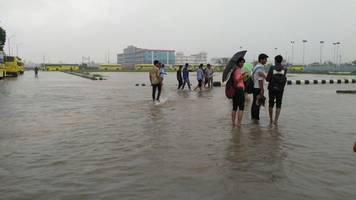
\includegraphics[scale=0.6]{images/ch/272.jpeg}
    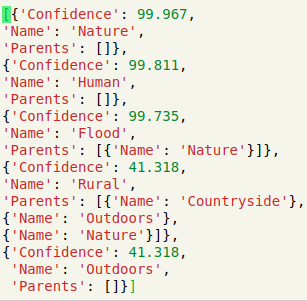
\includegraphics[scale=0.6]{images/ch/aws_272.png}
    \caption{Report image 272 and its top 5 AWS provided labels from Chennai
    2017 Dataset, Riskmap India}\label{fig:aws_272}
\end{figure}

The report image with id 1 from the Jakarta 2017 dataset was not taken during
heavy flooding. It depicts a drain that needs to be cleared ahead of the
monsoon season. Labeling the image shows that the labels are quite different and
that AWS correctly identifies the image as a ditch.
\begin{figure}[ht]
    \centering
    \captionsetup{justification=centering}
    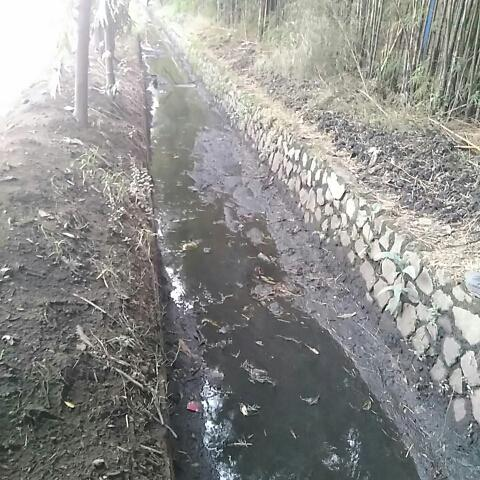
\includegraphics[scale=0.3]{images/id/1.jpeg}
    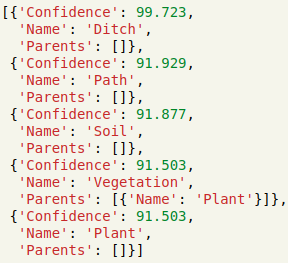
\includegraphics[scale=0.6]{images/id/aws_1.png}
    \caption{Report image 1 and its top 5 AWS provided labels from Jakarta
    2017 Dataset, Petabencana }\label{fig:aws_1}
\end{figure}


\subsubsection{Google Cloud Vision AI}
% here's what an image and the top 10 labels look like

Figure \figureautorefname{}~\ref{fig:goog_272} shows report image 272 as labeled
by the Google Cloud Vision AI API\footnote{The `mid' and `topicality' properties
have been redacted for brevity}.
\begin{figure}[ht]
    \centering
    \captionsetup{justification=centering}
    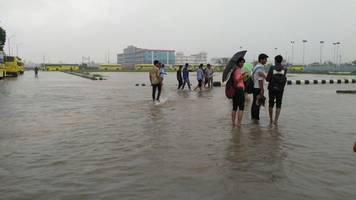
\includegraphics[scale=0.6]{images/ch/272.jpeg}
    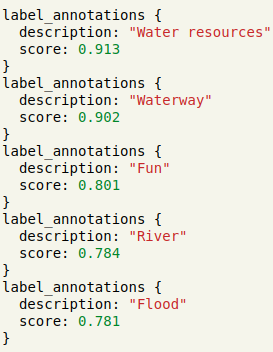
\includegraphics[scale=0.6]{images/ch/goog_272.png}
    \caption{Report image 272 and its top 5 Google Cloud Vision AI provided
    labels from Chennai 2017 Dataset, Riskmap India}\label{fig:goog_272}
\end{figure}

Whereas the top 5 labels from AWS are very distinct between Jakarta report 1 and 
Chennai report 272, the label annotations are quite similar for the response
from the Google API as shown in \figureautorefname{}~\ref{fig:goog_1}
\begin{figure}[ht]
    \centering
    \captionsetup{justification=centering}
    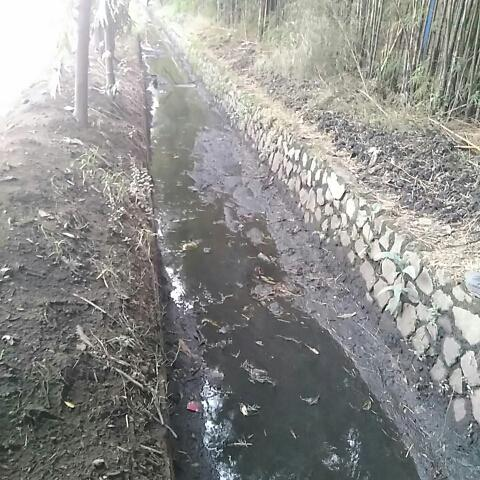
\includegraphics[scale=0.3]{images/id/1.jpeg}
    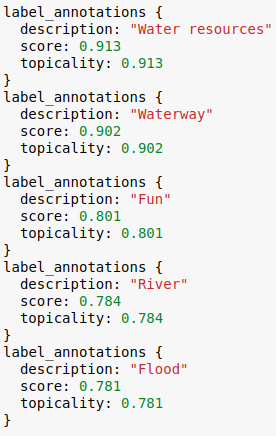
\includegraphics[scale=0.6]{images/id/goog_1.png}
    \caption{Report image 1 and its top 5 Google Cloud Vision AI provided
    labels from Jakarta 2017 Dataset, Petabencana}\label{fig:goog_1}
\end{figure}

% with zero labels and without
\subsection{Visual Bag of Words}
The bag of visual words as described in \sectionautorefname{}~\ref{chap3:image}
is used to create image embeddings out of the labels obtained from the
AwsLabeler or GoogleLabeler. Here a particular feature vector has a confidence
score at position i if the ith label in the vocabulary (created out of all
unique labels) is present in the
image~\cite{yangEvaluatingBagofvisualwordsRepresentations2007}.

\subsubsection{Results}
When the dataset size is limited and it is difficult to gather new data, 
it is possible to estimate future true error rates by using
cross validation. Cross validation consists of splitting the dataset into
k many groups. The learning model is then trained on k-1 groups and tested 
against the held out group. The average error over all k groups is then 
taken as an estimate of the true error rate of the model.
%TODO: table of perceptron and svm cross validation

With a balanced hold out set comprising of ten percent of the
data points, the Support Vector Machine (SVM) linear classifier achieves a score
upwards of \.70 as shown in \tablename{}~\ref{chap4:imageSvmPerceptron}.
Labels from AWS Rekognition were used because AWS returned many more labels than 
Google did for the same image. More labels means that there are more dimensions
for the classifier to differentiate between heavy flooding and no heavy flooding
images.

\begin{table}[htbp]
\centering
\caption{Image Classification Accuracy}
\label{chap4:imageSvmPerceptron}
\begin{tabular}{lllr}
\toprule
      Dataset &      Method &           Validation Method &  Validation Acc. \\
\hline
 Jakarta 2017 &  Perceptron &     10\% held out validation set &             0.70 \\
\midrule
 Jakarta 2017 &         SVM &     10\% held out validation set &             0.71 \\
 Chennai 2017 &  Perceptron &  mean 5 fold cross validation &             0.83 \\
 Chennai 2017 &         SVM &  mean 5 fold cross validation &             0.84 \\
\bottomrule
\end{tabular}
\end{table}


\section{Flood Height}
\subsection{Raw}
The flood height parameter was added as a raw feature. Since it was a scalar,
there were few degrees of freedom for a linear separator to split the space.
Attempting to create a decision tree on the flood height did not create a
predictor that could generalize well, neither on a held out validation set or
during cross validation with random shuffles; however, the inclusion of the raw
feature into the ensemble net increased performance as shown
in~\ref{chap4:ensemble_scores}.

\section{Ensemble with Neural Net}
In~\cite{jordanHierarchicalMixturesExperts1994}, Jordan and Jacobs showed that
neural networks can be effectively used to vote between different classifiers
that are effective only in their specific domain of the overall space. They present a
case for using several weak classifiers that have middling performance in order
to create a neural network that has better performance than any of the experts
it uses~\cite{jordanHierarchicalMixturesExperts1994}. Although Jordan and
Peterson formulated the problem as an extension of the EM algorithm and
therefore only used linear units, we use back propagation for training. This
choice was motivated by the desire to have an easy to modify network with
elements that may not be linear in the future. Furthermore, the compute savings
presented by Jordan and Peterson are less relevant now than in 1994~\cite{bishopPatternRecognitionMachine2006}.

We first train SvmLearners using the BowLabeler for text and either the AwsLabeler or
GoogLabeler for images. We then use the IdentityLearner in order to pass through
flood height as a raw feature. The results of these learners is synthesized into
a single feature vector by taking each applicable piece of data, creating its
embedding, and finding the signed distance from the learned separator to the
embedding. If the type of data for this separator doesn't exist, then that
feature is set to zero. In this way, each datapoint that is embedded into a
feature vector that has the same length as the number of Learners that were
trained.

% psuedo code or maybe real code 

\subsection{Validation Scores}~\label{chap4:ensemble_scores}
%TODO: THIS IS A PLACEHOLDER 
TODO: this a place holder --- will want to report std div of cross val + tidy up
the experiment jupyter notebooks. 10\% held out set is correct however.
\begin{table}
\centering
\begin{tabular}{llrlr}
\toprule
      dataset &              Learners &  size of hidden layer & mean 5 fold cross validation acc. &  10\% held out set \\
 Jakarta 2017 &         Aws,Bow,Flood &                     8 &                                xx &            0.7600 \\
\midrule
 Jakarta 2017 &               Aws,Bow &                     8 &                                xx &            0.8250 \\
 Jakarta 2017 &               Aws,Bow &                     9 &                                xx &            0.8375 \\
 Chennai 2017 &         Aws,Bow,Flood &                    10 &                                xx &            0.7300 \\
 Chennai 2017 &  Google,Aws,Bow,Flood &                    12 &                                xx &            0.8800 \\
 Chennai 2017 &               Aws,Bow &                    11 &                                xx &            0.7100 \\
\bottomrule
\end{tabular}
\end{table}

Where $\lambda{}$ is the mean 5 fold cross validation acc.
